I hated riding transport ships in space. Everything was too quiet, too peaceful. It didn't match the tension everyone was feeling. I'd much rather have rode into the Martian atmosphere and feel the rumble of re-entry.

{\it ETA to drop-point: 10 minutes}

`Thanks Sheut,' I said, breathing deeply. Years of experience and shock-absorbant casing meant drops had become easier for me. I breathed again, watching my chest guard rise and fall. The entire cockpit was designed to protect me, fully kitted with a chest guard, helmet and limb guards.

I willed the helmet to lower the blacked out visor so that I could focus on the Sarcoff's eyes. Through all the cameras around its body I could see the Gragt, the Calla, and the C-class FAA unit. The unit looked so small compared to the mechs. Where we stood even in drop mode at over 5 metres, the FAA's exosuits were barely taller than blue-G humans. Not that the exosuits did much, they gave the soldiers the ability to fly and some life support systems, but not much in the way of weaponry, too expensive. It wasn't as if the troops needed it; one of the Blue's treatments of the Federation colonists was to expose generations of Joops to mutagens. Due to being near the gas giant, it resulted in a society of high-Gs, a superhuman scourge to the low and blue-Gs.

But enhanced anatomy wouldn't stop Blue magic.

{\it ETA to drop-point: 10 minutes}

`I heard you the first time,' I responded.

I fidgeted under the chestplate, and glanced at the timer on my HUD. 3 minutes to drop.

3 minutes.

3, not 10. Not even close.

Sheut was looping.

I swore. How had this happened? When? He was working fine when we boarded the transport, and had kept updating me as we accelerated. I tried to open a private channel to Med'val. No luck. I could operate many of the Sarcoff's systems myself without Sheut's assistance, but not communications. I needed to stop Sheut from looping, otherwise I was going to die in drop, unable to make use of the thrusters to slow my descent.

{\it ETA to drop point: 10 minutes}

I tried to unhook my arm from the limb guard, but found that the locks were under Sheut's supervision, trapped in the loop. I was stuck. I turned my body as much as it could to face a screen to my left, a log that displayed everything Sheut had been doing. Being displayed were three lines that kept repeating. I couldn't turn around fully to see what they said, I could only see the ends of the lines.

-tem check

System check. Well that narrowed it down. I hoped the next two lines could do better than that.

-tional

Hell's fury, this wasn't working.

Then I felt a lurch in my stomach. I looked at my timer, it had turned green. 

We'd dropped.

{\it ETA to drop point: 10 minutes}

I prayed that the great Flow would deem me worth sparing, and looked at the last line.

-ing?

I was going to die. I would've started screaming, but I knew it didn't matter. The Sarcoff was airtight and shock absorbing. No one would be able to hear me as I screamed, burning and boiling.

I shakily chuckled, thinking that I'd finally earned the name of Coffin-rider.

\vspace{5mm}

{\bf {\large 3 hours ago...}}

`Who'll burn the Blue to ash, and claim it for the righteous?' shouted the lieutenant as he rallied his platoon.

`F-A-A!' came the reply. The soldiers chanted perfectly in time with each other. It was unnatural. Hell, their neural implants probably told them exactly when and how to cheer. Joops always knew how to take the fun out of something.

It was amusing to watch them getting ready to drop, considering how most of them were unlikely to come back from this operation. I nearly pitied them.

Nearly.

I was sitting up on a raised walkway above the repair stations. To the back of me was the inner hull. Nothing was there to stop people from falling off, so I just sat there dangling my legs over the edge, taking in the view of the mobilising army.

`Who's gonna drown them in their seas, and choke them in their air?'

`F-A-A!'

The FAA, the Federation Armed Alliance. An imposing force to be feared and revered, the pride and joy of the Jupiter Federation of Celestials. Or a mass of brainwashed orphaned high-Gs, used to wipe out any threats to the Federation, depending on who you asked.

`Sheut, progress report.'

I didn't hear a reply, I guessed I was out of range. I stood up, then hopped down to the top of my mech, the Sarcoff. A Tombstone-class Blite Industries Bipedal Shell, Pharoh variant. It wasn't pretty, the paint job was all but stripped away from years of use. Patches of gold and blue randomly torn off by bullets and damaged sections replaced by grey plating. But underneath that shielding it was angelic: high-output carbon muscle with micro-haptic sensors; nanite repair fluid running through every system; a versatile array of weapons and tools to get me past any enemy. Not to mention electromagnetic shielding, and an energy absorption field for counter-magic combat.

The cockpit door was open, perpendicular to the mech's back. It needed to be so that Sheut could talk to the maintenance crew. I could see the communications line running out from the mech. I used the ladder on the top of the Sarcoff to lower myself onto the door of the cockpit. The seat had been pulled out onto the rails of the door. It was in the way, and I needed to get closer for Sheut to be able to hear me.

`Sheut? Salsal?' I said, popping my head into the interior of the cockpit, manoeuvring around the seat.

{\it Salsal Ren, all bar three systems are at near-optimal functionality.}

The `voice' wasn't external but in my head, a signal transmitted from Sheut's core to my neural implants. Sheut was a CM, a Crystal Mind, a mineral lattice soul powered by the Flow of magic. I could see a light blink and flicker on Sheut's module, an integrated cylinder situated above where I would be sitting in the cockpit. It meant that he was `thinking', most likely about the specifications and repairs I'd told him to complete before drop.

`Let me guess, one of those three is the antenna?' I asked, exasperated by the sheer resistive nature of our shielding, a major selling point of the Pharoh. I first encountered one in the mines, where they were used to handle heavy equipment and resist the dangerous radiation of the minerals. I was assigned a bruised and battered Pharoh, a hunk of junk that would go on to become the Sarcoff I piloted today.

I returned my focus to the antenna, it looked foolish. Centuries of re-discovering and re-developing communication technology, and humanity still managed to mess up. Our own shielding hindering communications, Hell humanity deserved to be nearly wiped out.

Nearly.

{\it Correct, would you like to synchronise?}

`Yit, setting relay module up now,' I said, leaning down to the central control panel and flipping a switch.

{\it Synchronisation in 3, 2, 1, mark.}

Once synchronised, my HUD was activated, and my body felt small and weak. I could feel the power running through the Sarcoff, the individual fibres of synthetic muscle, the weapons readying to disengage safeties. Synchronisation linked Sheut's `mind' to mine, giving me more processing power at my disposal. It made it easier to use the extended nervous system, and gave me more options to control the Sarcoff's systems. I used to use a physical link, letting the Sarcoff hijack my nervous system and brain impulses to match the mech's systems instead. The integrated ports along my spine, arms and legs were a testament to that. But now that I had Sheut I didn't need them, the only implant I needed was the one in my head. But removing the ports could cause problems, and the Sarcoff's nervous system was still in use. So now the tech in my body and the link wires in the cockpit just gathered dust, the link wires themselves being tucked away in the cockpit.

Sheut gave me the general run down: antenna down, piledriver not functioning and a faulty thruster. I looked on the screen to my left to see what Sheut had been doing.

`Sheut, why did you deny installation for the FAA battery module?' I asked him out loud. No matter, he could choose how to listen to me.

{\it Analysis shows that although the module would be useful, the strain it would cause on the Sarcoff's coolant systems is not worth the extra power output.}

`Same issue with the old reactor?'

{\it Similar.}

`Alright, I'll trust your judgement. ETA on the specialist?'

{\it 3 minutes and 23 seconds.}

`Put up a countdown.'

On the top of my HUD a clock appeared. 3:21, 3:20, ...

{\it Update: if we abandon the piledriver module we can save another 20 minutes of repairs and be at optimal functionality at departure time.}

I sighed. As was typical of CMs, Sheut had a roundabout way of saying what he thought. Their restrictions on imperatives meant that they always had to seem subservient. The result: a passive aggressive backseat driver.

`Why do you not want the piledriver module? The Guild has done a full diagnostic on it to make sure it's actually useful, and we have no close range weaponry.'

{\it I am aware of the relevant data. However, I cannot help but notice that of our 114 operations across 7 years and 4 months of being partnered, and your further 5 years and 7 months of combat experience, you have only been in a position to make use of a close range weapon like the piledriver in a grand total of 5 cases.}

`So that's 5 times I could have used a weapon like this.'

{\it 2 of these cases were dealt with by stepping on the individual who attacked you.}

`And the other three?'

{\it Point blank harpoon shots.}

`Which isn't a close range weapon, it's impractical to rely on them like that.'

{\it Using the harpoons as close range weapons has made up 42.9\% of your total harpoon usage.}

I paused, did I really use them that little? I retorted with immaturity, knowing it would force him to be more direct.

`All the other Coffin-riders have CQC weapons! Drel uses a plasma lance!'

{\it Drel is a Hybrider, and specialises in close range and counter-mech combat. You on the other hand seem to specialise in clambering your way through every fight.}

We kept arguing, as per our unspoken agreement. Sheut and I were nervous. We had been given little to no information on the operation we had been assigned, apart from the fact that a C-class FAA unit was being assigned to us. C-class was good, which wasn't good news. The Federation made a point of never wasting resources, and they were willing to send a C-class unit and a Coffin-rider. So in times like these, Sheut and I would argue. It took the edge off.

`Ren!' shouted a gruff voice.

I clambered out of the cockpit and onto the top of my mech, my legs dangling over either side of the `head'. Ahead of me I could see Med'val, in his four legged heavy weaponry mech, the Gragt. It sported force-field generators in every nook and cranny of its overlapping and ornate plating.

`Salsal guildred!' I said, urging him to come over.

He complied, converting his mech into its mobile form. As it sunk its main body down and converted its legs into transport mode, Med'val laughed cheerily. This only got him the dirtiest of looks from the lieutenants of the FAA, unhappy to have this outlier to their protocol.

`How are you, my friend?' he asked me.

`Can't complain, risking my life for a cause I don't believe in, but getting paid for it!' I responded.

We laughed. Med'val and I were contractors, paid by the FAA to bolster their forces. The Jupiter Federation's policy against magic meant that their armies were all but ineffectual against magic. The FAA couldn't kit out all of the exosuits with counter-magic fields, far too expensive.

Enter the Guild, an independent organisation representing only the best warriors, everything from Spellswords to Coffin-riders. The Guild gave guys like Med'val and me backup, and a network of people to help us find jobs and to help us on those jobs, commonly known as the guildren. It was worth the small percentage taken off of you pay check to have the Guild on your side.

The FAA itself hated us. Anyone could ask for our services provided they had the money, so for idealists we were scum. It didn't help when a contractor like me used a CM. Even just making use of the natural Flow of magic was unacceptable to them.

At least it was meant to be, so much for their war against magic. The moment the Olympus War started, they begged the Guild for help. Both sides did.

`Well guildred, what brings you?' I asked him.

`Special operation, all very HUSH HUSH!' he said, tilting his head towards the lieutenants, very indiscreetly.

`You as well? If I didn't know any better, I'd say they were trying to get rid of us.'

He laughed, `As if they could win this war without Coffin-riders. When do you drop?'

`In just under an hour, dropping with C-class unit Lance.'

`You as well? Looks like we're teaming up, eh?' he grinned.

I froze, did I hear him right?

{\it You did, and the antenna is fully operational.}

I mentally thanked Sheut, and gathered my thoughts.

`They're sending two of the Guild's best Coffin-riders?' I asked.

`No. They're sending me, and you two as back up.'

We turned to see Drel's mech, a Hybrid. Not quite mechanical, not quite biological, Hybrid mechs were made by finding a young Demon. The creature from Hell was integrated into mech systems as it grew. Being treated to various mutagens and adjustments, as well as the DNA of the Coffin-rider, Hybrid mechs were among the best. Not only could they heal themselves, but also the pilot, and minimal signal delay from command to action didn't hurt either. The main positive was that a well-trained Hybrid could fight on its own, without a Hybrider. The drawback was that as the mech was alive, it needed to be cared for. Drel hated Demons, so instead of caring for hers, she dominated it.

Drel crawled out of the cockpit, a metal cocoon seemingly nailed into the creature's chest. She grinned as her mech, the Calla, put its `hand' in front of her so that she could be raised to the walkway. I could see the Calla shiver and warp under the translucent casing of its armour, just hiding the beast.

`Drel. Why do they need a Hybrider? Why would anyone need a Hybrider?' asked Med'val.

`To pick up the slack for you third rates!' she replied.

{\it Thruster: fully operational}

{\it Piledriver Specialist ETA: 15 seconds}

I ignored them, I was too deep in thought. We three were by far the best Coffin-riders in the Guild, making us the some of the most valuable assets to the FAA. No wasted resources, and they were sending all three of us along with a unit. These facts didn't worry my guildreds enough.

In my focused state, I hadn't noticed that the specialist had arrived, currently expecting a response to some greeting.

`You the specialist?'

`I am, I represent Blite Industries. I was told you were having configuration problems?'

`With the piledriver, yit.' I didn't like this guy, too happy. Didn't look like he'd ever even been in a fight, how was that possible?

`What seems to be the problem?' he said, smiling. What was there to smile about? Hell, I despised him.

`Every time it's activated, Sheut gets stuck in a feedback loop. Only way to free him is to disengage the piledriver.'

`Ah, have you considered giving it limited access to the module? We have fou-'

`Him,' I interrupted.

`I'm sorry?'

`Him, not it, him. Sheut has a fully developed personality matrix, male. Use the right words.'

`I apologise, it's just that most Shell Operators don't like the idea of a CM in their head.'

He knew Sheut could hear us, and yet still didn't talk to him. He was being disrespectful, either intentionally or by accident. I didn't like this guy, he'd insulted my partner. I started clenching my fist.

{\it May I take over this conversation, Ren? Preferably before you break his face.}

I breathed, `Go ahead, Sheut.'

A tone signalled the speakers of the Sarcoff turning on. The head turned to face the specialist, and a synthesised voice followed. He couldn't have seemed more uncomfortable having to talk directly to a CM. 

I chuckled to myself, and left them to it. I needed to find out more about the upcoming operation, I didn't want to drop when I felt this blind.

The lieutenants started to pretend that they were having an important discussion when they noticed me walking towards them. I got in close to their huddle, and put my arms onto the shoulders of the lieutenants closest to me.

`Salsal lieutenants, who knows anything about Lance team's oper-'

Suddenly a look of confusion passed over the faces of everyone in a small radius around me, 10 metres or so. They kept rubbing their eyes, tripping and trying to unblock their ears.

`-ation,' I finished, realising what had happened.

The FAA troops were fumbling around, trying to speak and taking cautious steps. Full deprivation capability. The neural implants of the FAA could act as a way of keeping confidential data hidden. It wouldn't have affected neural implants that weren't on the Federation's network, like Drel and Med'val. But to anyone who was standing near me, total sensory deprivation. The neural implants cut out their ability to feel, to see, to talk, to hear. Temporary oblivion.

I turned away and started heading back towards the Sarcoff. The sooner I left, the sooner the troops would return to normal. I had learned something though, deprivation-class security was only required by three types of operation: espionage, which we were too noticeable for; security of high level personnel, for which they wouldn't waste three Coffin-riders; or...

Amassing a force like this, I nearly pitied whoever we were going to kill.

Nearly.

\vspace{5mm}

{\bf {\large Present...}}

{\it ETA to drop point: 10 minutes}

Never realised how beautiful the flames of re-entry were. Safe for now in my mech, I decided to watch them peacefully.

A new countdown popped up on my HUD. 

`At current rate, approximately 116 seconds to landing.' It wasn't Sheut. It was his voice, but it was just reading off of the HUD, a simple system.

I'd burn up long before 116 seconds. To pass what time I had left, I explored the systems of the mech that I never got around to using. Servo combinations, haptic network, fuel economy subroutines, so many.

{\it ETA to drop point: 10 \&?)34?*vba\#ev8}

Sheut's light went out, I guess that the loop caused him to crash. Good for him, at least he won't be awake for his death.

I went back to the haptic network. The system that allowed my nervous system and the Sarcoff's to interact. I explored the old physical link network out of nostalgia, detecting all the connections under the mech's skin. I even saw the ones inside... the cockpit?

What in Hell?

{\it 100 seconds to landing.}

It took seconds to find the culprits. The link wires that I'd hidden away behind monitors and life support modules. I laughed, I hadn't needed the wires in so long. Then I noticed that one of the link wires was just behind me, to the right. A few inches from my right hand.

I froze.

{\it 90 seconds to landing.}

I told myself to not think. I reached out, and got a good grip under the module there. It was the catheter drain, put there so I would never have to touch it. I pulled, and it clattered onto the floor. I didn't check for leakage, plenty of time to worry about hygiene if I was alive.

I could see the entry node jutting out, I reached again. I could feel my fingertips brush onto the cold surface.

{\it 80 seconds to-}

`SHUT UP!' It was getting hotter in the cockpit. I needed to focus, so I strained every muscle I could to reach. My legs, my chest, I even pushed off the helmet with my neck.

I caught the wire between my fingertips, and pulled.

It slipped out.

`COME ON!' One more try, just one more. I silently prayed to any gods that would listen, and reached.

I caught the wire again, and this time I was surgical, carefully pulling it towards my wrist, to the nearest port. I eased it in, and it clicked.

I disengaged the drop mode, spreading the Sarcoff out as much as I could.

{\it 60 seconds to landing.}

The link wire I was connected to was for the port on my lower spine, not my wrist. The signals were all wrong. I didn't have time for this, so I used what control I had from the synchronisation to replace protocols for the link wires. I had no idea what kind of problems this would cause, but I was desperate.

{\it 50 seconds to landing.}

It was getting unbearably hot in here, and I needed to start decelerating. I activated the thrusters, the ones I had access to.

The two on the right side of the Sarcoff's back.

I started spinning, and ended up tipping downwards with the thrusters further accelerating my descent. A drip of sweat came from up my chest and onto my neck.

{\it Update: at current rate, approximately 20 seconds to landing.}

I couldn't afford to panic. Besides, my death was no longer certain, I could fight back. I could win.

I willed the wrist of the mech to move, causing the servos on the Sarcoff's back to activate, twisting it in mid-air. My back was now turned towards the ground, so I got the mech into position as best I could.

{\it 10 seconds to landing.}

I activated the thrusters, for a short burst. I repositioned, and blasted the thrusters again. I repeated the same pattern again and again, desperately slowing myself down.

{\it Update: at current rate, approximately 12 seconds to landing.}

I couldn't think, I was nearly passing out from the heat.

{\it Landing in 5... 4...}

I felt more alive now than I ever had.

{\it 3...}

I nearly regretted installing the piledriver.

{\it 2...}

Nearly.

{\it 1...}

\vspace{10mm}

\begin{figure}[h!]
\centering
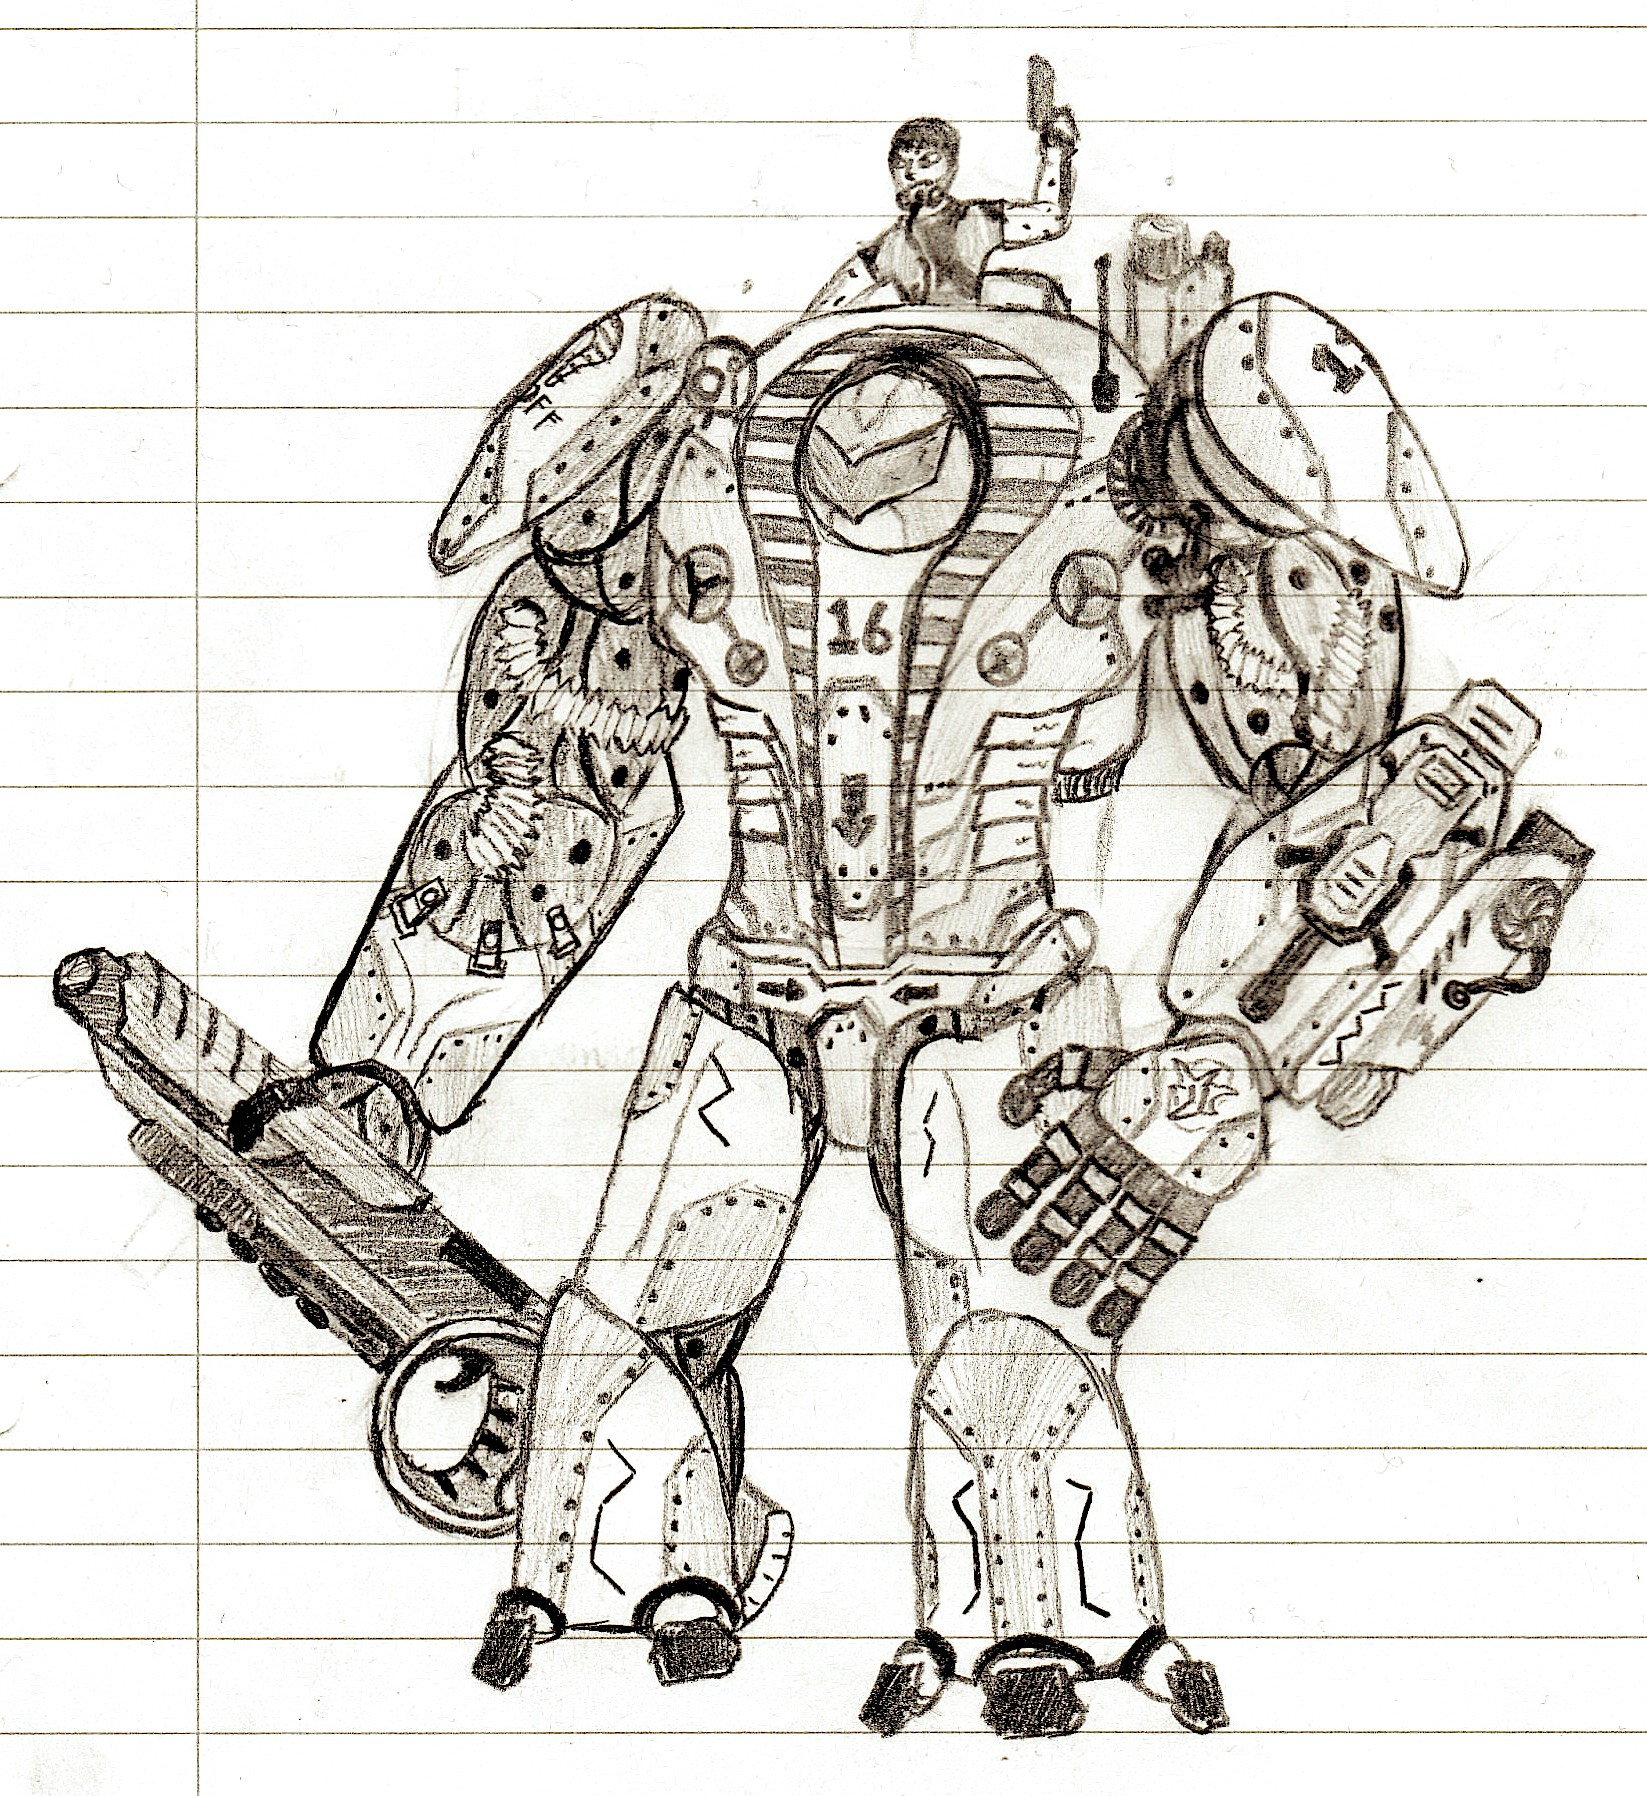
\includegraphics[width=0.9\textwidth]{./pictures/drop}
\end{figure}
